\chapter[Correção de erros, falhas e defeitos]{Correção de erros, falhas e defeitos}

\section{Visão Geral}
Ao longo do projeto diversos defeitos, erros e falhas foram corrigidos, a maioria deles no aplicativo móvel. Logo nas primeiras tentativas de rodar o aplicativo localmente, foram identificados problemas relacionados ao Expo, plataforma utilizada para o desenvolvimento do aplicativo mobile, que impediam os testes, geração de \textit{builds} e a sequência de desenvolvimento.

\textit{Build} é o processo de conversão de arquivos de código em uma versão executável. Esses artefatos, também podem ser chamados de \textit{builds}, e são o resultado final do processo de compilação. Então, o termo \textit{build} pode se referir tanto ao próprio processo de geração quanto ao produto gerado ao final.

Após as correções iniciais relacionadas ao Expo, os esforços foram concentrados na correção de defeitos relacionados às funcionalidades do Agromart. A API principal do sistema e a API Dicionário demandaram apenas algumas correções pontuais. Então a maior parte dos esforços foram direcionados para a correção de defeitos, erros e falhas no aplicativo móvel.

Essas correções simplificaram a estrutura do projeto, reduziram a complexidade no desenvolvimento e garantiram que o Agromart estivesse preparado para atualizações futuras de maneira mais simples e organizada. A integração com o EAS também proporcionou um fluxo de trabalho mais ágil para o desenvolvimento e a manutenção contínua do aplicativo.

\section{Erros relacionados à tipagem}
Ao longo do desenvolvimento foram identificados diversos erros de tipagem no aplicativo, que foram corrigidos para garantir melhor entendimento do código facilitando o desenvolvimento, reduzindo o tempo e esforço necessários para alterações no código fonte.

\subsection{TypeScript}
O TypeScript é uma linguagem de programação que adiciona algumas funcionalidades ao Javascript, como tipos e interfaces, permitindo que os desenvolvedores detectem erros durante o desenvolvimento. 

O uso do TypeScript traz vários benefícios, como menor probabilidade de erros por acesso de variáveis, propriedade, funções ou objetos não definidos e maior legibilidade e clareza do código.

Diferente de outras linguagens fortemente tipadas, o sistema de tipos do Typescript é usado para checar possíveis erros e avisos em tempo de compilação, já que o compilador pode identificar inconsistências e problemas de tipagem antes mesmo do código ser executado, por exemplo acesso a uma propriedade que pode possivelmente não estar definida em um objeto. 

Essa segurança não se propaga em tempo de execução, uma vez que o código Typescript é transpilado para Javascript antes de ser executado, e o JavaScript por sua vez tem a tipagem dinâmica. 

Isso explica o motivo desses erros de tipagem, apesar de gerarem confusão entre os desenvolvedores, não necessariamente causarão falhas em tempo de execução.

\subsection{Erros Corrigidos}
Para resolver esses problemas, primeiramente foi adicionado um \textit{script} de \textit{typecheck}, que verifica os erros de tipagem em todo o projeto e traz o endereço e a quantidade de erros de cada arquivo. Após rodar o \textit{typecheck}, foram quantificados 100 erros em 65 arquivos diferentes, como é possível ver nas Figuras \ref{erro-ts-1} e \ref{erro-ts-2}.

Para corrigir estes erros foram importadas bibliotecas de tipagens que deveriam estar sendo utilizadas, criação de interfaces para atributos sem qualquer tipagem, correção de interfaces incorretas que estavam causando conflitos, além da correção de partes do código que apresentavam erros na lógica e estavam sendo apontados pela tipagem.

Após a correção de todos estes erros relacionados ao TypeScript, o \textit{typecheck} foi rodado novamente eliminando todos eles, como se pode ver na Figura \ref{ts-corrigido}. Como resultado, todos os 100 erros dos 65 arquivos diferentes foram corrigidos.

\begin{figure}[h]
	\centering
	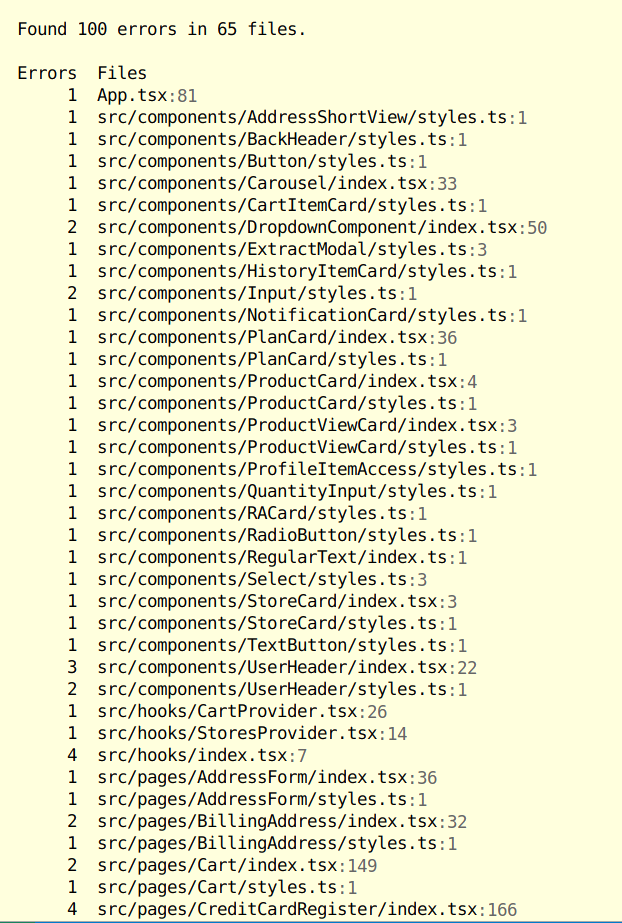
\includegraphics[keepaspectratio=true,scale=0.4]{figuras/tserros1.png}
	\caption{Primeira imagem de erros do TypeScript}
	\label{erro-ts-1}
\end{figure}

\begin{figure}[h]
	\centering
	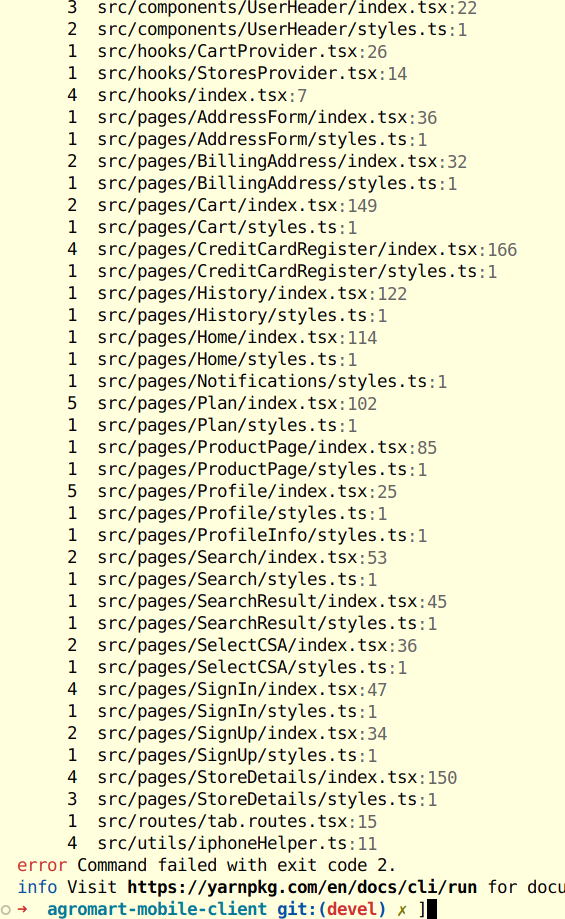
\includegraphics[keepaspectratio=true,scale=0.4]{figuras/tserrors2.png}
	\caption{Segunda imagem de erros do TypeScript}
	\label{erro-ts-2}
\end{figure}

\begin{figure}[h]
	\centering
	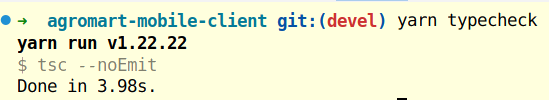
\includegraphics[keepaspectratio=true,scale=0.4]{figuras/tscorrigido.png}
	\caption{Typecheck após correções}
	\label{ts-corrigido}
\end{figure}


\section{Falhas e erros relacionados a versões depreciadas ou incompatíveis e funcionalidades nativas}
\subsection{Aplicativo ejetado}

O Agromart foi inicialmente construído utilizando o Expo, uma plataforma que facilita o desenvolvimento de aplicativos mobile ao fornecer ferramentas e bibliotecas prontas para uso. No entanto, o aplicativo estava configurado de forma ejetada, ou seja, ele havia sido removido de alguns dos sistemas de conveniência do Expo para possibilitar a utilização de recursos nativos que o Expo não oferece suporte. No caso do Agromart, essa ejeção foi desnecessária, pois o aplicativo não utilizava nenhum recurso nativos adicional. Essa configuração acabou introduzindo complexidade desnecessária ao projeto, desorganizando os diretórios e tornando o processo de desenvolvimento mais complexo.

Ter um Aplicativo ejetado estava causando diversos problemas para gerar uma \textit{build} de produção realmente funcional, como erros de parâmetros do java, erros diversos de compilação e incompatibilidade de versões. Especificamente para o Agromart, um Aplicativo ejetado pode ser um grande causador de problemas, pois é um Aplicativo que não recebe manutenção tão frequentemente, e com o tempo podem surgir erros de \textit{build} no Android quando novas atualizações do Expo são lançadas.

Para resolver esse problema, e além disso, proporcionar um ambiente de desenvolvimento mais simples e produtivo para o Agromart, foi criada uma nova versão do projeto, sem a ejeção, utilizando a versão da SDK 49 do Expo. A SDK é um conjunto de ferramentas e bibliotecas que os desenvolvedores usam para construir e manter o aplicativo.

Além disso, uma conta no EAS (Expo Application Services) foi criada para o nosso projeto Agromart, note que a criação dessa conta não afeta nem possui relação com quaisquer outras contas criadas anteriormente para o aplicativo, pois utilizamos um nome de pacote diferente do original do Agromart, de forma que nosso projeto fique apartado. O EAS é um serviço do Expo que permite a gestão de \textit{builds} e atualizações do aplicativo de forma centralizada e eficiente, facilitando o processo de desenvolvimento. Com o novo projeto configurado e o código do Agromart migrado para a SDK 49, todas as bibliotecas foram atualizadas para garantir a compatibilidade com a nova versão. Isso permitiu que o primeiro APK do aplicativo (arquivo de instalação utilizado em dispositivos Android) fosse gerado com sucesso na nova versão, resolvendo problemas de compatibilidade e trazendo maior organização ao projeto.

\subsection{Padronização de gerenciamento de pacotes}

Houve também a padronização do gerenciador de pacotes, o aplicativo do Agromart estava utilizando dois gerenciadores de pacotes diferentes, o NPM e o Yarn, e isso é uma má pratica. Por conta disso o arquivo \texttt{npm.lock} foi removido para manter apenas o \texttt{yarn.lock}, simplificando o gerenciamento das dependências do projeto. Além disso, uma série de bibliotecas foram atualizadas com as novas versões, e foi realizada a migração de bibliotecas que não eram mais suportadas, evitando problemas futuros de manutenção.

\subsection{Expo Doctor}

O Expo disponibiliza uma ferramenta chamada Expo Doctor, onde é possível visualizar problemas com o projeto, foram corrigidos todos os problemas que existiam, pois estavam nos impedindo de gerar versões de produção. Como podemos ver na Figura \ref{doctor-fail} , existiam muitos problemas de compatibilidade de versões e de bibliotecas instaladas. Já na Figura \ref{doctor-success} vemos o comando rodando sem detectar nenhum problema após as correções efetuadas.

\begin{figure}[h]
	\centering
	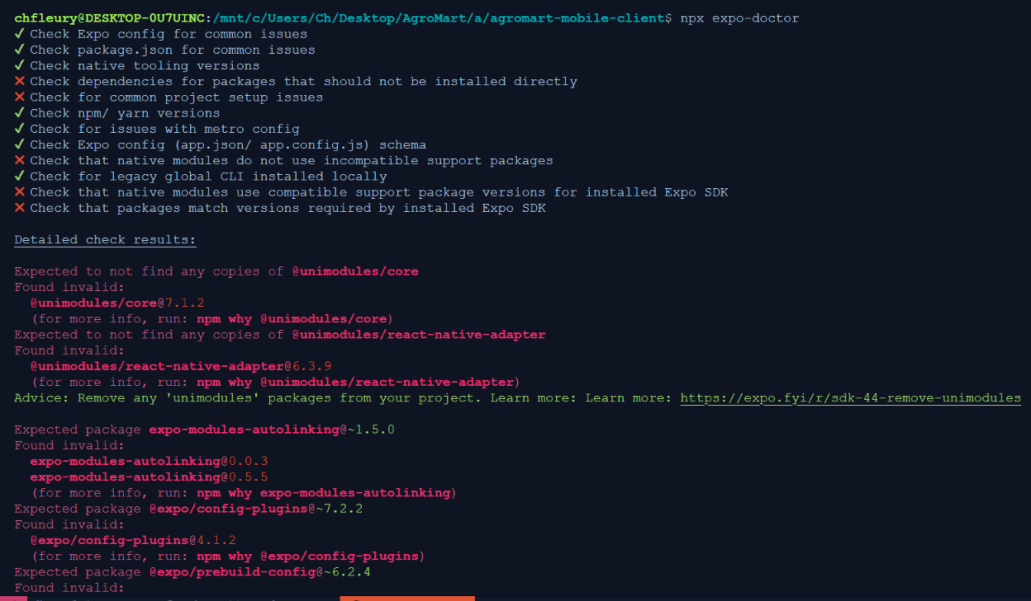
\includegraphics[keepaspectratio=true,scale=0.5]{figuras/doctor-fail.png}
	\caption{Problemas encontrados pelo Expo Doctor}
	\label{doctor-fail}
\end{figure}

\begin{figure}[h]
	\centering
	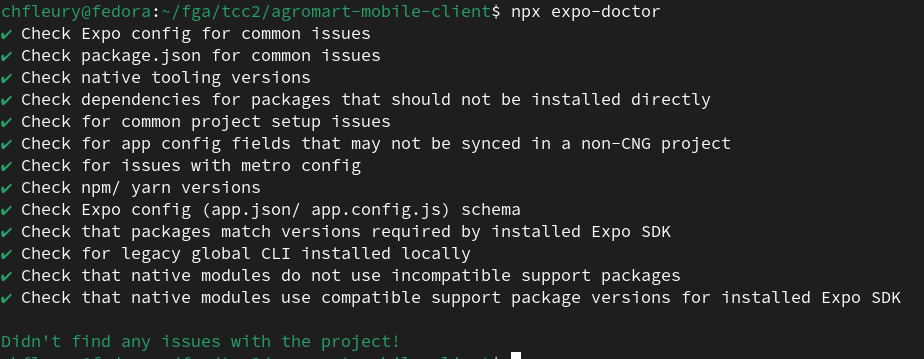
\includegraphics[keepaspectratio=true,scale=0.4]{figuras/doctor-success.jpeg}
	\caption{Expo Doctor sem problemas após correções}
	\label{doctor-success}
\end{figure}

\subsection{Problemas detectados após publicação}

Além dos problemas detectáveis pelo Expo ou momento de compilação do projeto, existiam alguns erros em tempo de execução que eram causados por bibliotecas, como um \textit{crash} no aplicativo que ocorria apenas em \textit{builds} de produção causado por uma biblioteca depreciada, como mostrado na Figura \ref{react-reanimated-crash}.
\textit{Crash} se refere a uma falha abrupta que causa o fechamento do aplicativo móvel de repente. No defeito aqui descrito, o \textit{crash} ocorria na tela de carregamento ao abrir o aplicativo. Esse problema só foi devidamente diagnosticado graças a uma versão de teste interno que foi publicada na loja antes da versão final de produção, através dela tivemos acesso ao relatório de causas de \textit{crash} de aplicativo da Google Play Store, possibilitando a sua correção.
Mais informações sobre o processo de publicação de versões de teste interno e sua importância podem ser encontradas no Capítulo 6 deste trabalho (ver seção de Publicação).

\begin{figure}[h]
	\centering
	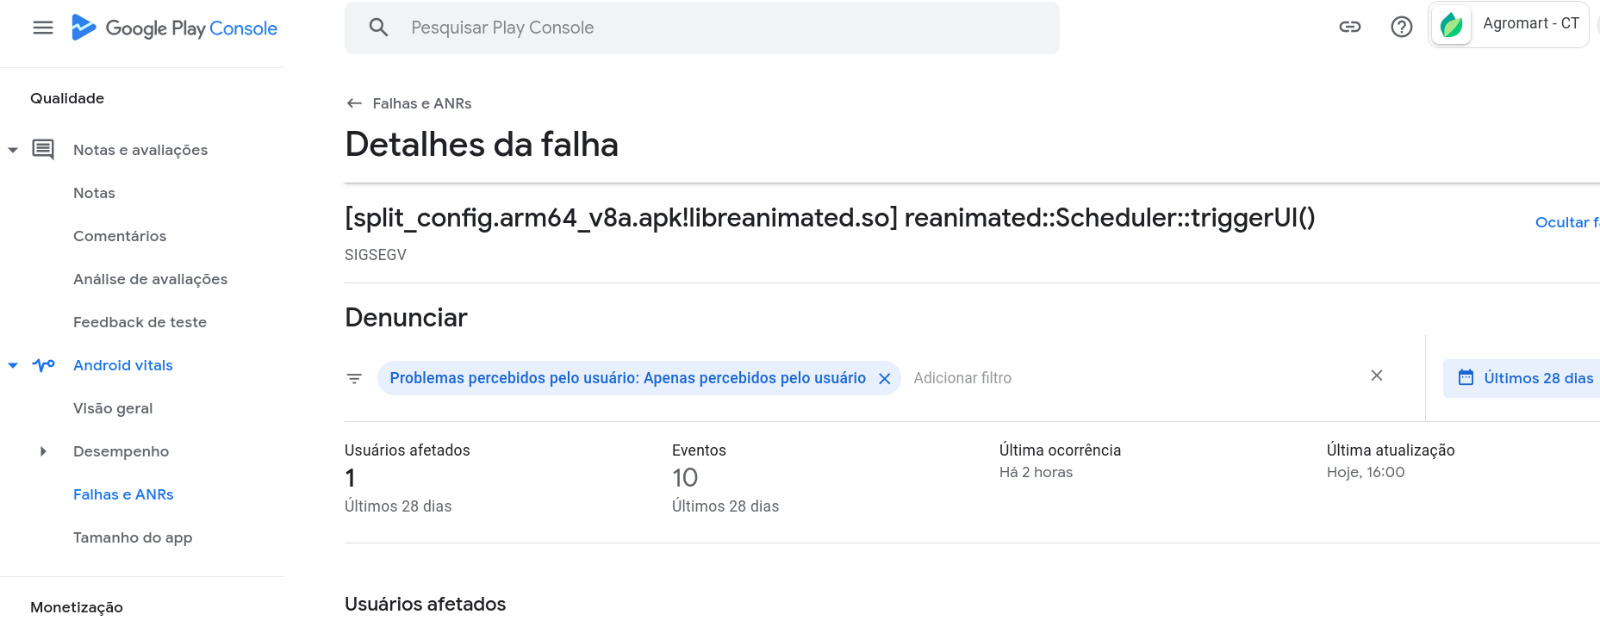
\includegraphics[keepaspectratio=true,scale=0.4]{figuras/react-reanimated-crash.png}
	\caption{Report de Crash causado pela biblioteca react-reanimated}
	\label{react-reanimated-crash}
\end{figure}

\section{Defeitos relacionados à funcionalidades do Agromart}
Durante o desenvolvimento do aplicativo Agromart, foram realizadas diversas correções para garantir o correto funcionamento das funcionalidades essenciais do MVP.

\subsection{Alterações no aplicativo móvel}

Inicialmente, foi corrigido o uso da URL base da API Dicionário, que estava comprometendo a seleção da CSA ao iniciar o aplicativo. Essa URL base deveria agora apontar para a API Dicionário que nós fizemos o deploy, visto que outros deploys da API dicionário feitos em semestres anteriores não estavam mais acessíveis.

Uma das correções mais importantes foi a padronização das chamadas de API de CSAS, pois em algumas telas, algumas chamadas eram feitas incorretamente para a API Dicionário, quando na verdade, deveriam ser feitas para a API da CSA selecionada. Também foi resolvido um problema relacionado ao \textit{token} de autenticação, que afetava a comunicação entre o aplicativo móvel e o backend das CSAs.

Além disso, foram solucionados \textit{crashes} na tela de histórico e na tela de pedidos, e um defeito que causava a exibição incorreta de compras de valor zero no histórico, como mostrado na Figura \ref{historyzero}.

\begin{figure}[h]
	\centering
	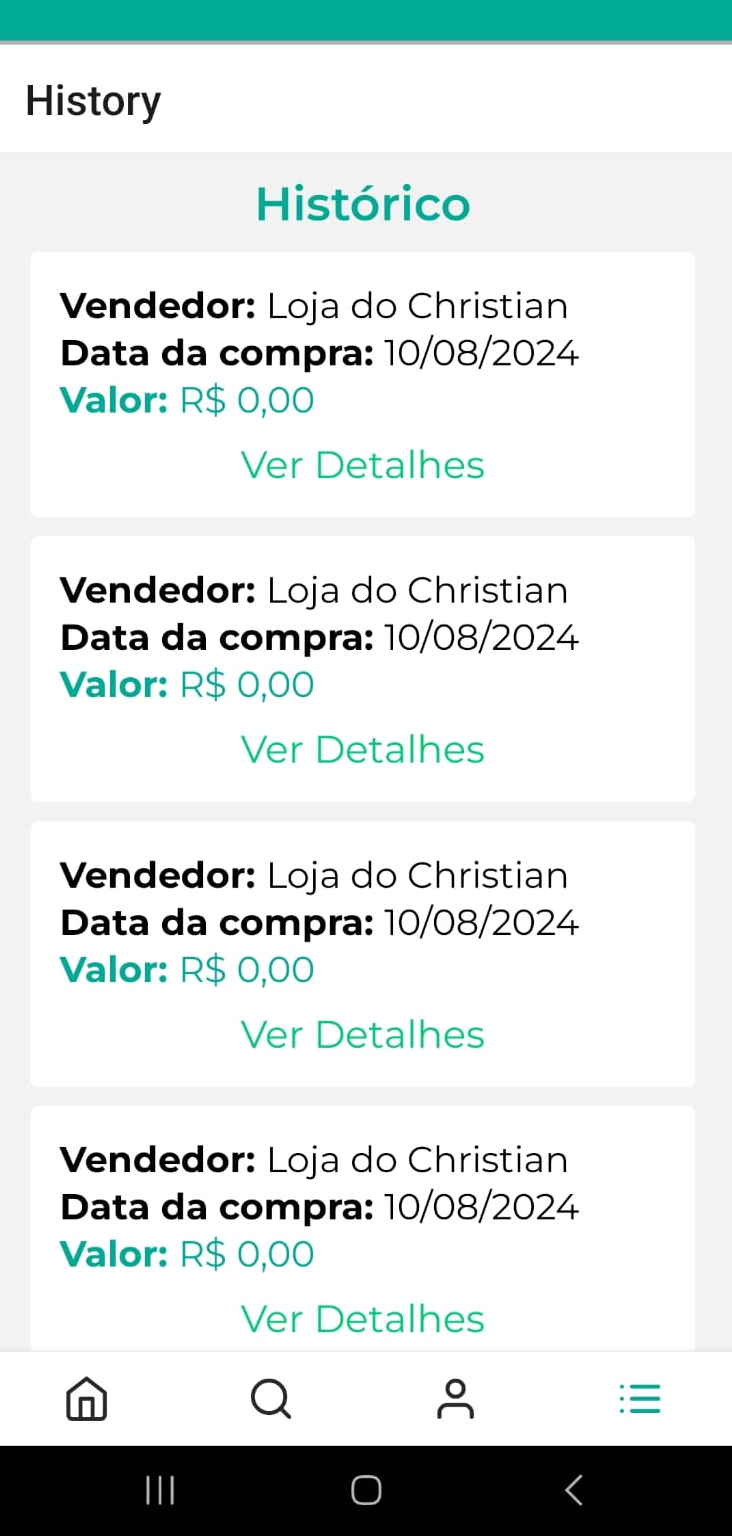
\includegraphics[keepaspectratio=true,scale=0.4]{figuras/historyzero.png}
	\caption{Histórico exibindo todas as compras com valor de R\$ 0,00}
	\label{historyzero}
\end{figure}

O redirecionamento após o login foi ajustado para garantir que os usuários fossem direcionados corretamente para a tela inicial após se logarem no aplicativo.

Erros relacionados à cadastro e edição do endereço do usuário também foram corrigidos, como vemos na Figura \ref{enderecoerro} era exibido um erro que não tinha relaçao com endereço e não era possível cadastrar um endereço de usuário pelo aplicativo nem edita-lo posteriormente.

\begin{figure}[h]
	\centering
	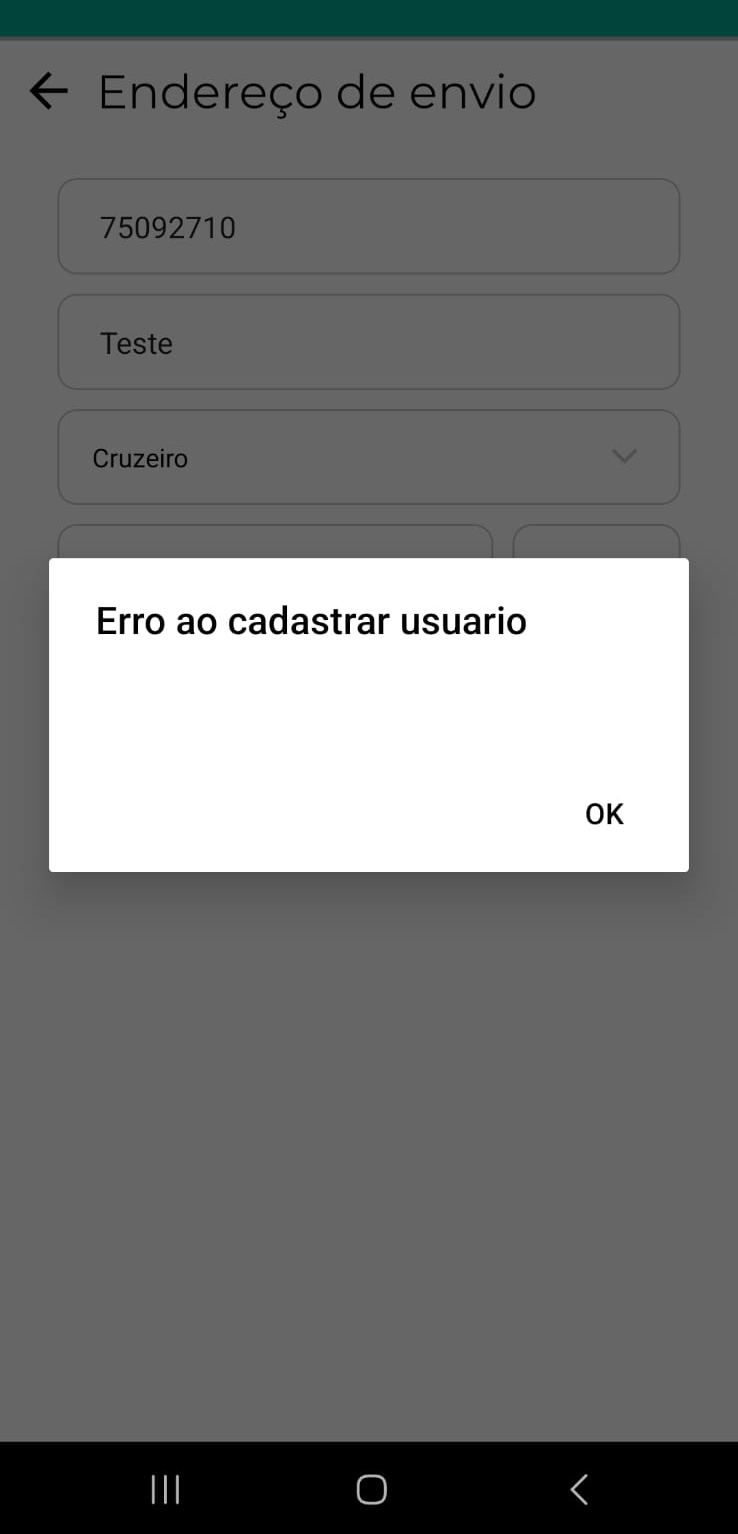
\includegraphics[keepaspectratio=true,scale=0.4]{figuras/enderecoerro.png}
	\caption{Erro ao cadastrar usuário na tela de cadastro de endereço}
	\label{enderecoerro}
\end{figure}

Também houveram diversas correções de erros em tempo de execução causados por problemas de tipagem, acessos de propriedades que não estavam definidas, ou de fontes que não eram encontradas, como visto na Figura \ref{erros}.

\begin{figure}[h]
	\centering
	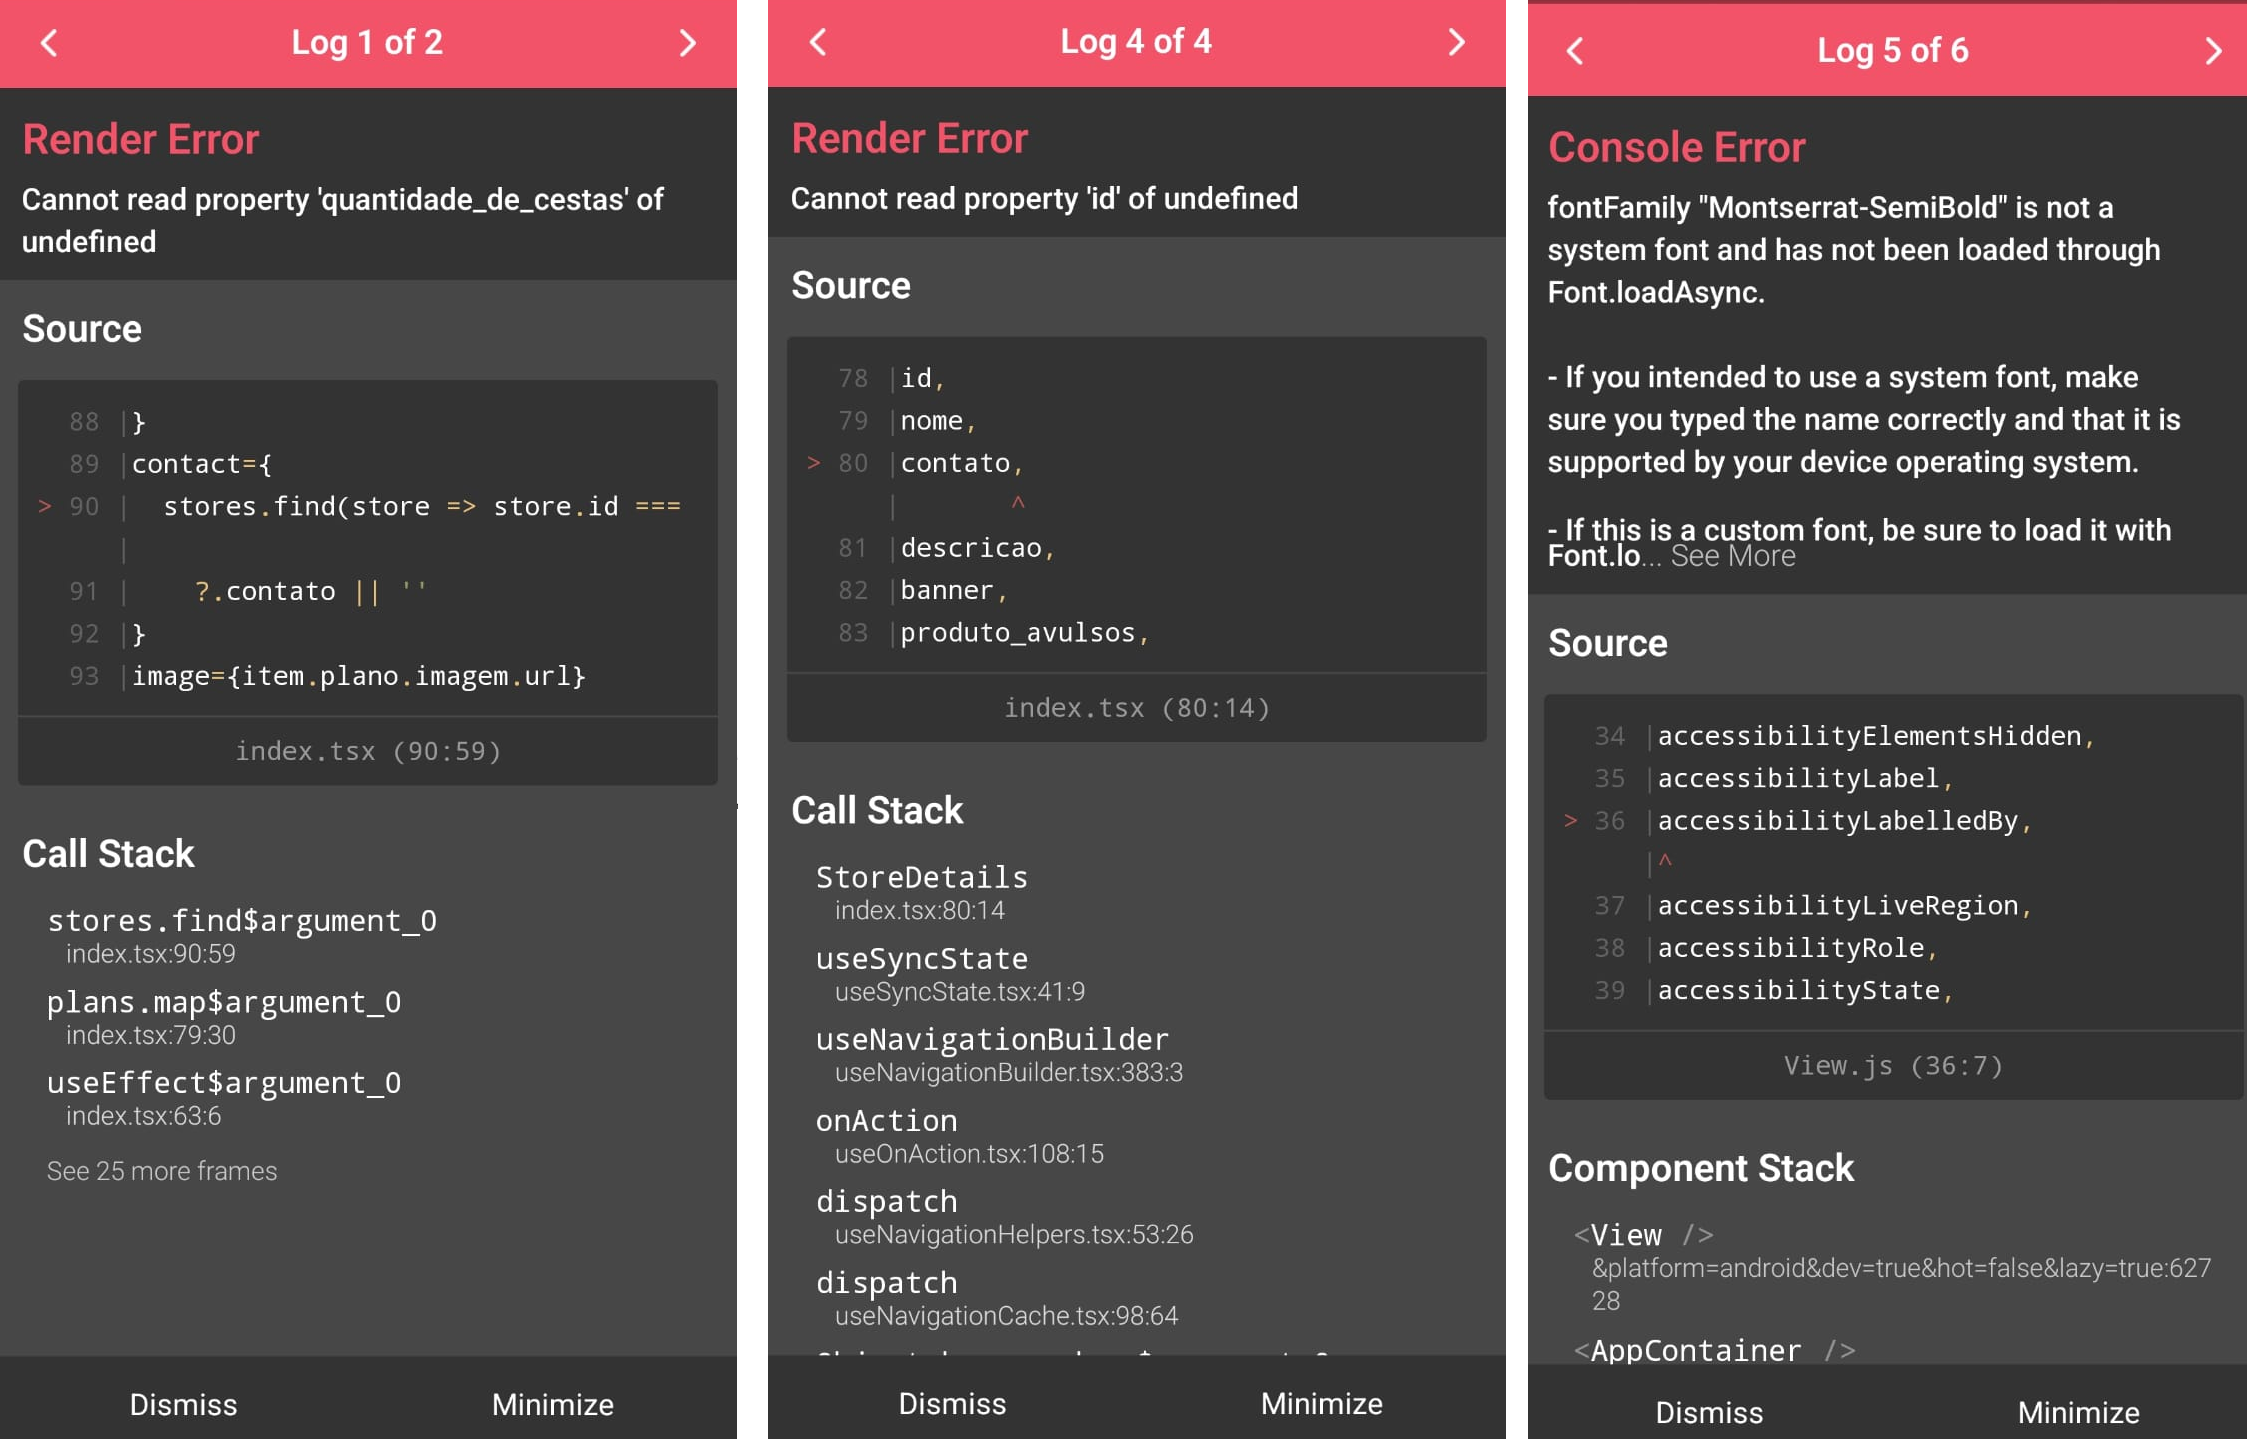
\includegraphics[keepaspectratio=true,scale=0.2]{figuras/erros.png}
	\caption{Compilação de erros de execução}
	\label{erros}
\end{figure}

Outras correções incluíram a resolução de um problema em que o Aplicativo tentava fazer a listagem adequada das lojas antes do login, o que não funcionava pois a URL base da CSA ainda não estava configurada. Melhorias na exibição de imagens em todo o aplicativo e a correção do filtro de histórico de compras. Também foi corrigido um problema relacionado à assinatura de planos, que anteriormente não salvava corretamente qual plano o usuário tinha assinado.

Essas correções foram essenciais para garantir uma experiência de uso fluida e confiável no Agromart.

\subsection{Funcionalidade de pagamento por cartão de crédito}
A funcionalidade de pagamento por cartão de crédito no Aplicativo, em vez de ser corrigida, foi desabilitada, uma vez que apresentava problemas críticos em ambiente de produção, impossibilitando com que pudéssemos receber pagamentos corretamente pelas plataformas do Mercado Pago ou PayPal. Foi tentado integrar a CSA fictícia que criamos com uma conta real do Mercado Pago, para que os pagamentos fossem feitos em ambiente de produção, porém apesar dos esforços, a funcionalidade não foi integrada corretamente.

Além disso o fluxo de pagamentos impedia a realização de qualquer pedido sem que fosse feito o pagamento por cartão adiantado pelo aplicativo, não possibilitando que fossem utilizados quaisquer outras formas de pagamento, como em dinheiro ou cartão na hora da entrega, o que compromete a usabilidade do aplicativo, e poderia frustrar tanto os usuários quanto as CSAs.

Dado esse cenário, a abordagem adotada foi de desabilitar essa funcionalidade, mas sem perder nenhum código que foi desenvolvido, o código apenas não é mais acessado. Dessa forma, o fluxo de pedidos fica mais simples e funcional, com o pedido sendo criado com pagamento pendente, podendo ser pago de formas flexíveis como na entrega, em dinheiro, PIX ou qualquer outro meio de pagamento aceito pela CSA. Uma vez pago e/ou entregue, esses status podem ser atualizados pela administração da CSA no painel.

\subsection{Alterações no Backend e na API dicionário}
As principais correções necessárias se concentraram no aplicativo móvel, nas outras partes do sistema não houve a necessidade de muitas correções.

No Backend do Agromart foi realizada uma correção na exibição das imagens das cestas de produtos. Que não eram retornadas na resposta da requisição.

\subsection{Pull-requests geradas e lista de alterações}

Ao final de todo o trabalho, foram geradas duas \textit{pull-requests}, já com todas as correções aplicadas, bem como código unificado de todas as \textit{branches} existentes nos repositórios.

A \textit{pull request} acessível em \url{https://github.com/AgroMart/api/pull/81} contém o código resultante da unificação das \textit{branches} existentes no repositório e da correção de um defeito na exibição de imagens de cestas e produtos na API.

A \textit{pull request} acessível em \url{https://github.com/AgroMart/mobile-client/pull/17} contém o código resultante da unificação das \textit{branches} existentes no repositório do aplicativo e também das seguintes correções: 

\begin{itemize}
    \item Unificação das \textit{branches} do aplicativo
    \item Correção no endpoint da API Dicionário
    \item Ajuste no uso da UrlBase proveniente do dicionário
    \item Correção no \textit{token} de autenticação para a AGROMART-API
    \item Padronização do gerenciador de pacotes, removendo \texttt{npm lock} e mantendo apenas \texttt{yarn.lock}
    \item Criação de novo projeto com Expo na SDK 49, eliminando a necessidade de ejetar o aplicativo
    \item Migração do código do aplicativo para o novo projeto na SDK 49
    \item Atualização das bibliotecas compatíveis
    \item Migração de bibliotecas não suportadas
    \item Geração do primeiro APK após a atualização para SDK 49
    \item Correção de falha de \textit{crash} na tela de histórico
    \item Correção de defeitos relacionados à compras de valor zero no histórico
    \item Correção de \textit{crash} na tela de pedidos
    \item Ajuste no redirecionamento após login para a tela inicial
    \item Desativação do fluxo de pagamento por cartão de crédito
    \item Atualização das URLs no aplicativo
    \item Correção de defeito onde o aplicativo tentava listar lojas antes do login
    \item Correções na tela de planos
    \item Mensagem de "Erro ao cadastrar usuário"\ na criação/edição de endereço
\end{itemize}
